This chapter will describe how we implemented the simulator. The simulator consists of four separate parts: \\
\begin{enumerate}
	\item Scanner
	\item Parsing
	\item Contextual Analyzer
	\item Interpretation
\end{enumerate}

\paragraph{The scanner} scans through the teamfiles and the config file, and builds token out of keywords. It simply goes from one character to another, and everytime it can put characters together to a predefined keyword/terminal it saves it as a token for the parser to use.


\begin{figure}[H]
\centering
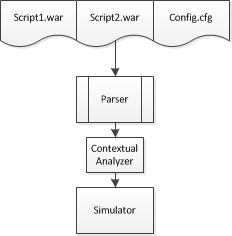
\includegraphics[scale=1.2]{rapport/6/figures/script_to_simu}
\label{fig:script_to_simu}
\caption{From scripts to simulation}
\end{figure}

To give a roughly picture of how the scripts gets interpret and outputted to the simulator we have made a rough drawing that shows how it all works in the big picture figure \ref{fig:script_to_simu}

\section{Parser construction}
	In this section we will describe how one can construct a parser from a EBNF, but first we will describe what a parser is and how it works.
	
	\subsection{Parsing strategies}
		The job of a parser is to check if a program is syntactically correct and 
		to determine the structure of the program. To do this we constructed an {\it abstract syntax tree}.
		There are two common ways of checking this {\it Bottom-up Parsing} and {\it Top-Down Parsing}, that are explained next.
		
		\subsubsection*{Bottom-up Parsing}
			This way of parsing takes simple structures and combining them to more complex structures.
			This type of parsing is commonly called {\it LR parsing} because we read the text from the left and reduces to the right.
			\begin{figure}[H]
				\centering
				\subfloat[Top down]{\label{fig:top_down}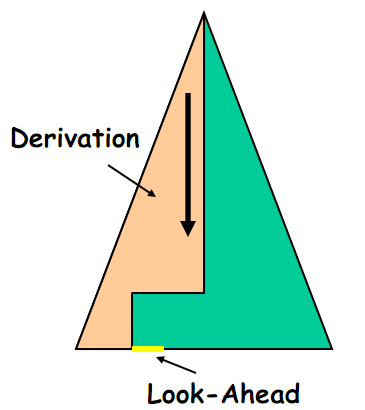
\includegraphics[width=0.4\textwidth]{rapport/6/figures/topdown}} 
				\subfloat[Bottom up]{\label{fig:bottom_up}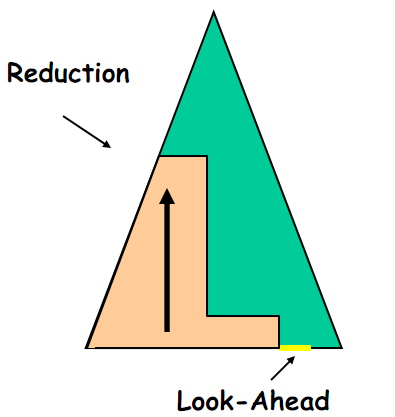
\includegraphics[width=0.4\textwidth]{rapport/6/figures/bottomup}}
				\caption{Two different parse methods:Top-down(LL) on the left and bottom-up(LR) on the right}\label{fig:parsers}
			\end{figure}
			
		\subsubsection*{Top-down Parsing}
			Top-down parsing figure \ref{fig:top_down} starts from the complex structures, and breaks them down into smaller parts.
			This type of parsing is commonly called {\it LL parsing} because we read the text from the left and make derivations to the left.
		
		\subsubsection*{Strengths and weaknesses}
			The most commonly used parsing strategy of the two is LR parsing, the reason for this is because it is faster than LL parsing.
			In this project, however we have chosen to make a LL parser because it's easy to implement, furthermore speed is not important for us. 
			The type of LL parser we made is called a recursive descent parser.
			
	\subsection{A recursive descent parser}
		A recursive descent parser is a LL parser which works by recursively going through the program code.
		To construct this type of parser a EBNF is required and here is how it is made:
		\begin{enumerate}
			\item Make a scanner for reading chars and identifying them as terminals.
			\item Make a parse method for each non-terminal in the EBNF.
			\item Make a method that can accept terminals.
			\item In each of the parse method accept terminals and/or call other parse methods.
		\end{enumerate}		
	
	\subsection{Abstract Syntax Tree}
		The structure of the parsed program is stored as a AST. The tree structure is called abstract because it doesn't contain the concrete
		structure of the EBNF, but rather a abstract representation of the source code. Because of this there isn't a straightforward way to 
		construct such a tree. We constructed the AST-structure by making node classes for each terminal, declaration, control structure and making these 
		reference each other similar to how a non-terminals, in the EBNF references its right-hand side terminals and non-terminals.
		
		